\section{Task 5}


\begin{figure}[H]
\centering
\begin{circuitikz}[american voltages]

    % Nodes
    \node[circle, draw=black, fill=none, thick, inner sep=2pt] (Vtop) at (-3,1.5) {};
    \node[circle, draw=black, fill=none, thick, inner sep=2pt] (Vbot) at (-3,-1.5) {};

    \node[circle, fill=black, inner sep=0pt] (N1) at (-1,1.5) {};
    \node[circle, fill=black, inner sep=0pt] (N2) at (2,1.5) {};
    \node[circle, fill=black, inner sep=0pt] (N3) at (2,-1.5) {};
    

    % Voltage source
    \draw (Vtop) to[vsourcesin, l=$10\sin(2\pi 50 t)$] (Vbot);

    % Bottom rail
    \draw (Vbot) -- (N3);

    % Series resistor
    \draw (Vtop) -- (N1)
          to[R=$R_1$] (N2);

    % Top wire to load
    \draw (N2) -- ++(3,0) coordinate (TopR);
    \draw (N3) -- ++(3,0) coordinate (TopB);

    \draw (TopR) -- ++(3,0) coordinate (Vt);
    \draw (TopB) -- ++(3,0) coordinate (Vb);

    \draw (Vt) to[open, v=$U_0$] (Vb);

    % Zener diode branch
    \draw (N3) to[zzD, l=$Z_1$, a=$6.8V$] (N2);

    % Load resistor
    \draw (TopR) to[zzD, a=$Z_2$, l=$3.9V$] (TopB);

\end{circuitikz}
\caption{}
\end{figure}

\noindent
Since we have diodes in both directions of a parallell, and they both have zenor voltages higher than $0.7V$. Regarding current direction and voltage, one zenor will open and the other turn on. That means that maximum voltage potential difference over the parallell branch is $\pm 0.7V$. We can graph $U_0(t)$ and $U_i(t)$.

\begin{figure}[H]
\centering
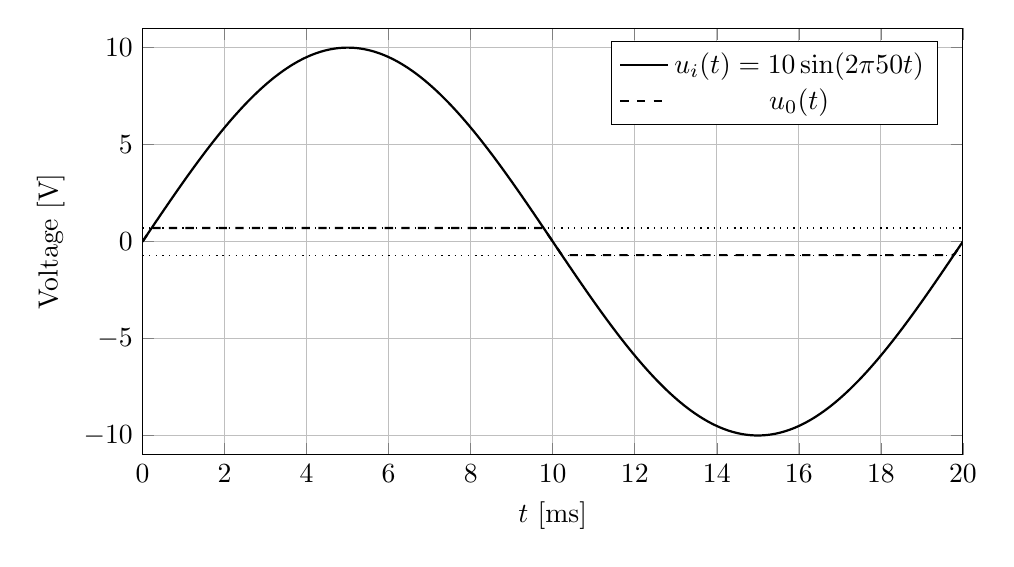
\begin{tikzpicture}
\begin{axis}[
    width=12cm,
    height=7cm,
    xlabel={$t$ [ms]},
    ylabel={Voltage [V]},
    xmin=0, xmax=20,
    ymin=-11, ymax=11,
    grid=both,
    legend pos=north east,
    domain=0:20,
    samples=400
]

% Input
\addplot[thick]
{10*sin(deg(2*pi*50*x/1000))};
\addlegendentry{$u_i(t)=10\sin(2\pi 50t)$}

% Output
\addplot[thick, dashed]
{
(10*sin(deg(2*pi*50*x/1000)) > 0.7) * 0.7
+
(10*sin(deg(2*pi*50*x/1000)) < -0.7) * (-0.7)
+
and(10*sin(deg(2*pi*50*x/1000)) >= -0.7, 10*sin(deg(2*pi*50*x/1000)) <= 0.7)
* (10*sin(deg(2*pi*50*x/1000)))
};
\addlegendentry{$u_0(t)$}

% Reference lines
\addplot[dotted] {0.7};
\addplot[dotted] {-0.7};

\end{axis}
\end{tikzpicture}
\caption{Input and clipped output voltage.}
\label{fig:zener_clipping}
\end{figure}

\noindent
The circuit will have no flowing current whenever the diodes are open circuit. When $| U_0(t) | > 0.7V$, there will be current flowing. The absolute max current is as below.

\[
I_{tot\uparrow} = \frac{10V - 0.7V}{1k\Omega} = 9.3mA
\]

\noindent
The graph of the current is as shown under.

\begin{figure}[H]
\centering
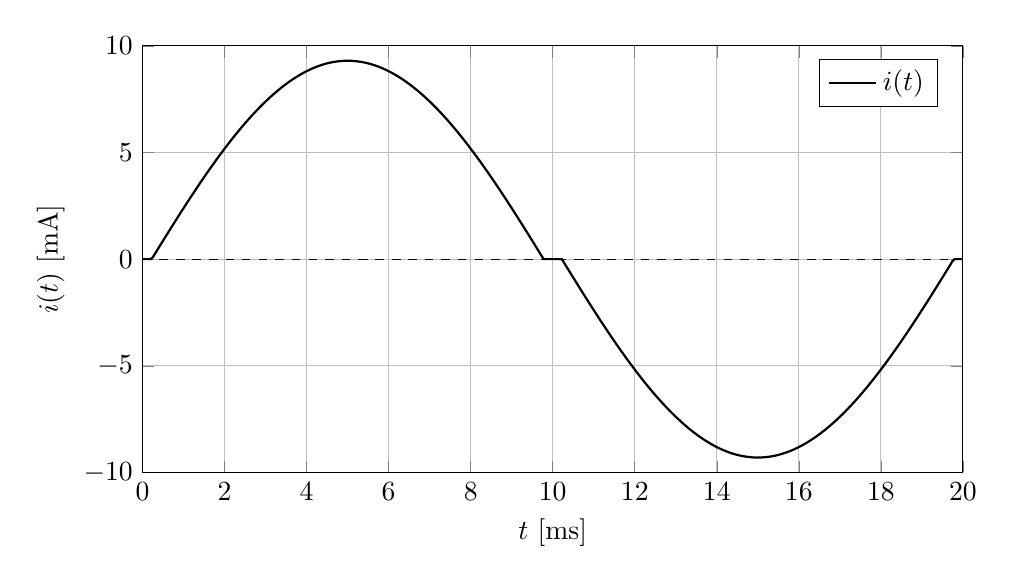
\begin{tikzpicture}
\begin{axis}[
    width=12cm,
    height=7cm,
    xlabel={$t$ [ms]},
    ylabel={$i(t)$ [mA]},
    xmin=0, xmax=20,
    ymin=-10, ymax=10,
    grid=both,
    legend pos=north east,
    domain=0:20,
    samples=400
]

% Current (mA)
\addplot[thick]
{
1000 * (
(10*sin(deg(2*pi*50*x/1000)) > 0.7)
* ((10*sin(deg(2*pi*50*x/1000)) - 0.7)/1000)
+
(10*sin(deg(2*pi*50*x/1000)) < -0.7)
* ((10*sin(deg(2*pi*50*x/1000)) + 0.7)/1000)
)
};
\addlegendentry{$i(t)$}

% Zero line
\addplot[dashed] {0};

\end{axis}
\end{tikzpicture}
\caption{Current with diode threshold.}
\label{fig:current_plot_signed}
\end{figure}